\documentclass{article}
\usepackage{booktabs}
\usepackage{graphicx}
\title{Compression Module}
\author{Justin}
\date{}
\begin{document}
   \maketitle
   \section*{Algorithm}
   \begin{enumerate}  
   \item Divide input data into segments equivalent to 20 to 40\% of the available memory. (Larger buffer size)
   \item Divide the segments into variable chunks for data de duplication. 
   \item De duplicate chunks based on fingerprinting and hashing techniques.
   \item Supply the de duplicated chunks to a Diff tree generator: this generates a maximum spanning tree based on the diffability among chunks (All pair shortest path approach). Uses the root as the base for diff ( Needs a little clarification) .
   \item Do a delta compression using the root from the above step, and arrange the data into a single continuous block for final compression.
   \item Do a final compression on the block generated from above step (lz or bzip2).
\end{enumerate}  
   \begin{figure}[!th]
    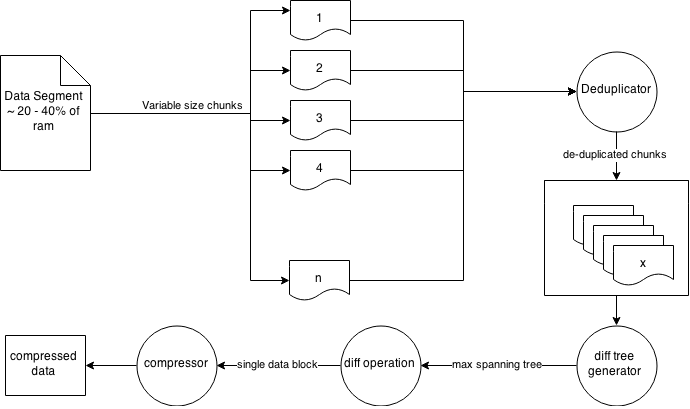
\includegraphics[scale=0.5]{compressor.png}
   \end{figure}
\end{document}

